\documentclass[12pt]{exam}
\newcommand{\hwnumber}{8}
\newcommand{\hwname}{Hash Tables and Binary Search Trees}

%%% begin hw-packages-and-macros.tex
\usepackage{amsmath}
\usepackage[left=1in, right=1in, top=1in, bottom=1in]{geometry}
\usepackage{graphicx}
\usepackage{hyperref}
\usepackage{color}
\usepackage[all]{xy}
\usepackage{wrapfig}
\usepackage{fancyvrb}
\usepackage[T1]{fontenc}
\usepackage{listings}
\usepackage{ctex}

\newcommand{\fillinlistings}{
    \lstset{ %
    language=C, numbers=left, numberstyle=\footnotesize, stepnumber=1,
    numbersep=4pt, showspaces=false, showstringspaces=false, tabsize=4,
    breaklines=true, breakatwhitespace=false,
    basicstyle=\normalsize\fontfamily{fvm}\selectfont, columns=flexible,
    mathescape=true, escapeinside={(*}{*)},
    morekeywords={alloc, allocarray, assert},
    otherkeywords={@requires, @ensures, @loop_invariant, @assert}
    }
}
\newcommand{\normallistings}{
    \lstset{ %
    language=C, numbers=left, numberstyle=\footnotesize, stepnumber=1,
    numbersep=4pt, showspaces=false, showstringspaces=false, tabsize=4,
    breaklines=true, breakatwhitespace=false,
    basicstyle=\footnotesize\fontfamily{fvm}\selectfont, columns=flexible,
    mathescape=true, escapeinside={(*}{*)},
    morekeywords={alloc, allocarray, assert},
    otherkeywords={@requires, @ensures, @loop_invariant, @assert}
    }
}

\newcommand{\semester}{Spring 2014}

\newcommand{\Cnought}{C$0$}
\newcommand{\modulo}{\ \texttt{\%}\ }
\newcommand{\lshift}{\ \texttt{<<}\ }
\newcommand{\rshift}{\ \texttt{>>}\ }
\newcommand{\cgeq}{\ \texttt{>=}\ }
\newtheorem{task}{Task}
\newtheorem{ectask}{Extra Credit Task}
\newtheorem{exercise}{Exercise}

\newcommand{\answerbox}[1]{
\begin{framed}
\hspace{5.65in}
\vspace{#1}
\end{framed}}

\pagestyle{head}

\headrule \header{\textbf{15-122 Written Homework \hwnumber}}{}{\textbf{Page
\thepage\ of \numpages}}

\pointsinmargin \printanswers

\setlength\answerlinelength{2in} \setlength\answerskip{0.3in}
%%% end hw-packages-and-macros.tex

\begin{document}

\addpoints
\begin{center}
\textbf{\large{15-122 : Principles of Imperative Computation, \semester
\\  \vspace{0.2in} Written Homework~\hwnumber
}}

 \vspace{0.2in}

 \large{Due before class: Thursday, March 20, 2014}
\end{center}

\vspace{0.5in}

\hbox to \textwidth{Name:\enspace\hrulefill}


\vspace{0.2in}

\hbox to \textwidth{Andrew ID:\enspace\hrulefill}

\vspace{0.2in}

\hbox to \textwidth{Recitation:\enspace\hrulefill}


\vspace{0.5in}

\noindent The written portion of this week's homework will give you some
practice working with hash tables, priority queues and heaps.
You can either type up your solutions or write them
\textit{neatly} by hand, and you should submit your work in class on the
due date just before lecture begins. Please remember to \textit{staple}
your written homework before submission.
\vspace{0.2in}

\begin{center}
\gradetable[v][questions]
\end{center}

\vspace{0.2in}
\begin{center}
  \Large{You must do this assignment in one of two ways and bring the stapled
         printout to the handin box on Thursday:

\bigskip
    1) Write your answers \textit{neatly} on a printout of this PDF.

\bigskip
    2) Use the TeX template at
    \url{http://www.cs.cmu.edu/afs/cs.cmu.edu/academic/class/15122-s14/www/theory8.tgz}
 }
\end{center}


\newpage
\begin{questions}


\question{\textbf{Hash Tables: Data Structure Invariants}}

Refer to the \Cnought{} code below for \texttt{is\_ht}
that checks that a given hash table \texttt{ht} is a valid hash table.
\begin{verbatim}
struct chain_node {
  elem data;
  struct chain_node* next;
};
typedef struct chain_node chain;

struct ht_header {
  chain*[] table;
  int m;     // m = capacity = maximum number of chains table can hold
  int n;     // n = size = number of elements stored in hash table
};
typedef struct ht_header* ht;

bool is_ht(ht H) {
  if (H == NULL) return false;
  if (!(H->m > 0)) return false;
  if (!(H->n >= 0)) return false;
  //@assert H->m == \length(H->table);
  return true;
}
\end{verbatim}

An obvious data structure invariant of our hash table is that every
element of a chain hashes to the index of that chain.
This specification function is incomplete, then:
we never test that the contents of the hash table
hold to this data structure invariant. That is, we test only on the
struct \texttt{ht}, and not the properties of the array within.

You may assume the existence of the following client functions as
discussed in class:

\begin{verbatim}
int hash(key k);

bool key_equal(key k1, key k2);

key elem_key(elem e)
//@requires e != NULL;
  ;
\end{verbatim}

\newpage
\begin{parts}
\part[4]
Extend \texttt{is\_ht} from above, adding code to check
that every element in the hash table matches the chain
it is located in, and that each chain is non-cyclic.

\begin{solution}
\begin{verbatim}
bool is_ht(ht H) {
  if (H == NULL) return false;
  if (!(H->m > 0)) return false;
  if (!(H->n >= 0)) return false;
  //@assert H->m == \length(H->table);

  int nodecount = 0;

  for (int i = 0; i < H->m; i++)
  {
    // set p equal to a pointer to first node
    // of chain i in table, if any

    chain* p = H->table[i];

    while (p != NULL)
    {
      elem e = p->data;

      if ((e == NULL) || (hash(elem_key(e)) != i))

        return false;

      nodecount++;

      if (nodecount > H->n)

        return false;

      p = p->next;

    }
  }

  if (nodecount != H->n)

    return false;

  return true;
}
\end{verbatim}
\end{solution}

\part[1]
Consider the \texttt{ht\_lookup} function given below:

\begin{verbatim}
elem ht_lookup(ht H, key k)
//@requires is_ht(H);
{
  int i = abs(hash(k) % H->m);
  chain* p = H->table[i];
  while (p != NULL)
  //@loop_invariant is_chain(p, i, H->m);
  {
    //@assert p->data != NULL;
    if (key_equal(elem_key(p->data), k))
      return p->data;
    else
      p = p->next;
  }
  /* not in chain */
  return NULL;
}
\end{verbatim}

Give a simple postcondition for this function.

\begin{solution}
\begin{verbatim}
/*@ensures \result == NULL

           || key_equal(k, elem_key(\result));
@*/
\end{verbatim}
\end{solution}

\end{parts}

\newpage
\question{\textbf{Binary Search Trees}}

\begin{parts}
\part[1]
Draw the binary search tree that results from inserting the following keys in the order given:

\begin{verbatim}
75  92  99  13  84  42  71  98  73  20
\end{verbatim}

Be sure all branches in your tree are clearly drawn so we can distinguish left branches from right branches.

\begin{solution}

  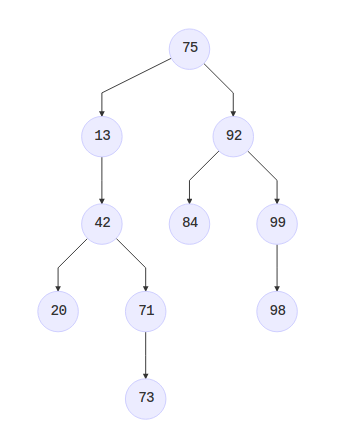
\includegraphics[scale=0.6]{BST.png}
\end{solution}

\part[1]
How many different binary search trees can be constructed using the following five keys:
\texttt{73, 28, 52, -9, 104} if they can inserted in any arbitrary order?

\begin{solution}
首先插入73时,104只能作为右子树插入,左子树树根为28后有一种情况,其余均两种,共5种。\\
首先插入28时,情况与插入73一致,共五种。\\
首先插入53时,左右子树各两种情况,共四种。\\
首先插入-9或104时,数的数量相同,以-9为例。插入-9后,只存在元素个数为4右子树,无论选取哪个元素作为树根,右子树个数与第一种情况相同,共4*5=20种。\\
综上所述,共54种。
\end{solution}
\newpage
Refer to the implementation of binary search trees discussed in class that is available on our course website.


\part[3]
Write an implementation of a new library function, \texttt{bst\_height}, that returns the height of a binary search tree. The height of a binary search tree is defined as the maximum number of nodes as you follow a path from the root to a leaf. As a result, the height of an empty binary search tree is 0. Your function must include a \textbf{recursive} helper function \texttt{tree\_height}.

HINT: In general, the height of a tree rooted at node T is one more than the height of its deepest subtree.

\begin{solution}

\begin{verbatim}
int tree_height(tree* T)
//@requires is_ordered(T, NULL, NULL);
//@ensures T == NULL || \result > 0
{
  if (T == NULL) return 0;
  if (tree_height(T->left) > tree_height(T->right))
    return 1 + tree_height(T->left);
  else 
    return 1 + tree_height(T->right);
}

int bst_height(bst B)
//@requires is_bst(B);
//@ensures is_bst(B);
{
  return tree_height(B->root);
}
\end{verbatim}

\end{solution}

\newpage
\part[5]
Consider extending the BST library implementation with the following function which deletes an element from
the tree with the given key.
\begin{verbatim}
void bst_delete(bst B, key k)
//@requires is_bst(B);
//@ensures is_bst(B);
{
        B->root = tree_delete(B->root, key k);
}
\end{verbatim}

Complete the code for the recursive helper function \texttt{tree\_delete} which is used by the \texttt{bst\_delete} function. This function should return a pointer to the tree rooted at \texttt{T} once the key is deleted (if it is in the tree).

You will need to complete an additional helper function \texttt{largest\_child} that removes and returns the largest child rooted at a given tree node T.

\begin{solution}

\begin{verbatim}
tree* tree_delete(tree* T, key k)
{
    if (T == NULL) {   	               // key is not in the tree

        return NULL;

    }

    if (key_compare(k, elem_key(T->data)) < 0) {

       T->left = tree_delete(T->left, k);

       return T;

    } else if (key_compare(k, elem_key(T->data)) > 0) {

       T->right = tree_delete(T->right, k);

       return T;

    } else {      // key is in current tree node T

        if (T->left == NULL)        // node has only right child

            return T->right;

        else if (T->right == NULL)   // node has only left child

            return T->left;

        else {         // Node to be deleted has two children

            if (T->left->right == NULL) {

                // Replace the data in T with the data
                // in the left child.

                T->data = T->left->data;

                // Replace the left child with its left child.

                T->left = T->left->left;

               return T;
            }
            else {
                // Search for the largest child in the
                // left subtree of T and replace the data
                // in node T with this data after removing
                // the largest child in the left subtree.
                T->data = largest_child(T->left);
                return T;
            }
        }
    }
}

elem largest_child(tree* T)
//@requires T != NULL && T->right != NULL;
{
    if (T->right->right == NULL) {

        elem e = T->right->data;

        T->right = NULL;

        return e;
    }

    return largest_child(T->right);
}
\end{verbatim}
\end{solution}



\end{parts}



\end{questions}

\end{document}
